\chapter{High-Performance Hybrid Architecture}

\section{System Constraints and Asymptotic Complexity}

The Monte Carlo simulation of Geometric Brownian Motion, while mathematically elegant, introduces severe computational bottlenecks when scaled to millions of trajectories. In a standard purely-interpreted environment (such as Python with NumPy), the SDE is vectorized iteratively as described by the standard literature \cite{hilpisch2018python}. 

While NumPy array broadcasting accelerates execution compared to standard Python loops, it forces an asymptotic memory complexity of \(\mathcal{O}(N)\). Simulating \(10000000\) trajectories allocates simultaneous RAM space for all intermediate normal variables \(Z\), asset prices \(S_T\), and option payoffs. This continuous memory allocation destroys L1/L2 CPU cache (ultra fast memory for data access) hits and introduces severe risks of \textit{Out of Memory} (OOM) errors on consumer hardware.

Our engine resolves this by recalculating the stochastic paradigm in an optimized C++ core. The \texttt{MonteCarloPricer} abstraction simulates random variables, computes the terminal price \(S_T\), extracts the payoff, and accumulates it into an atomic sum on-the-fly, purging memory immediately. This ensures a strict \textbf{\(\mathcal{O}(1)\) space complexity}, enabling the simulation of billions of paths with a constant, minimal memory footprint.

\begin{figuresrs}[red!5!white]
\begin{tikzpicture}[
    scale=0.85, transform shape,
    node distance=1.5cm and 3cm,
    block/.style={rectangle, draw=black!80, fill=white, thick, text width=4cm, align=center, rounded corners, minimum height=1cm},
    arrow/.style={->, thick, >=stealth}
]
    % Python O(N) side
    \node (pytitle) [font=\bfseries] {Python / NumPy: $\mathcal{O}(N)$};
    \node (pyarray) [block, below=0.5cm of pytitle, minimum height=3cm] {Array of $N$ paths\\ \vspace{0.2cm} \small{{[Path 1]} \\ {[Path 2]} \\ \dots \\ {[Path N]}} \\ \vspace{0.2cm} \textbf{High RAM usage}};
    \node (pyram) [block, fill=red!10, below=0.5cm of pyarray] {RAM Exhaustion Risk};

    \draw [arrow] (pytitle) -- (pyarray);
    \draw [arrow] (pyarray) -- (pyram);

    % C++ O(1) side
    \node (cpptitle) [font=\bfseries, right=3.5cm of pytitle] {C++ Engine: $\mathcal{O}(1)$};
    \node (cpploop) [block, below=0.5cm of cpptitle, minimum height=1cm] {On-the-fly calculation loop};
    \node (cppacc) [block, fill=green!10, below=1cm of cpploop] {Atomic Accumulator\\(Scalar Value)};
    
    \draw [arrow, loop right, distance=1.5cm, in=30, out=-30] (cpploop.east) to node[right, align=center] {Calculate \& \\ Discard} (cpploop.east);
    \draw [arrow] (cpploop) -- (cppacc) node[midway, right] {Add};
    \draw [arrow] (cpptitle) -- (cpploop);
    % Connection / comparison
    \draw[thick, dashed, gray] (3.8, 0.5) -- (3.8, -6); % separator line
    
\end{tikzpicture}
\caption{Memory Footprint Comparison: NumPy Vectorization vs C++ On-The-Fly Accumulation}
\end{figuresrs}
\clearpage 
\section{System Architecture Design}

To harness both Python's flexibility for research and C++'s bare-metal performance, the system is designed around a decoupled, two-layer hybrid architecture.

\begin{figuresrs}[red!5!white]
    \includegraphics[width=0.9\textwidth]{../architecture/component_diagram.pdf}
    \caption{Component Level Architecture of the Pricing Engine}
\end{figuresrs}

The core domain logic (Pricing Methods, Market Data, and the European Option representations) is fundamentally modeled using Object-Oriented Programming (OOP). For example, the \texttt{MarketData} struct acts as an immutable data container, while \texttt{MonteCarloPricer} encapsulates the numerical simulation mechanics as stateless methods. The C++ backend leverages these encapsulated objects to ensure type safety and high performance during the mathematical loops.

Furthermore, this structural division adheres to the \textbf{SOLID} principles of software design:
\begin{itemize}
    \item \textbf{Single Responsibility Principle (SRP):} Financial domain logic (e.g., computing a \texttt{EuropeanOption} payoff) is completely isolated from the numerical integration logic (\texttt{MonteCarloPricer}).
    \item \textbf{Open/Closed Principle (OCP) \& Dependency Inversion (DIP):} The high-level Monte Carlo engine depends solely on abstract interfaces, remaining closed to modification while open to extension via polymorphism.
    \item \textbf{Liskov Substitution Principle (LSP):} Derived classes maintain strict mathematical contract compliance, ensuring the core engine behaves deterministically regardless of the specific derivative passed to it.
\end{itemize}
\clearpage

\begin{landscape}
    Specifically, the design utilizes the \textbf{Strategy Pattern} to abstract the payoff logic. By defining a common interface for the option's payoff mechanism, the Monte Carlo engine remains completely decoupled from the specific type of derivative being priced. This architectural decision ensures the pricing engine is easily extensible to future, more complex exotic options (e.g., Barrier or Asian options) without altering the highly optimized simulation core.

\begin{figuresrswide}[red!5!white]
    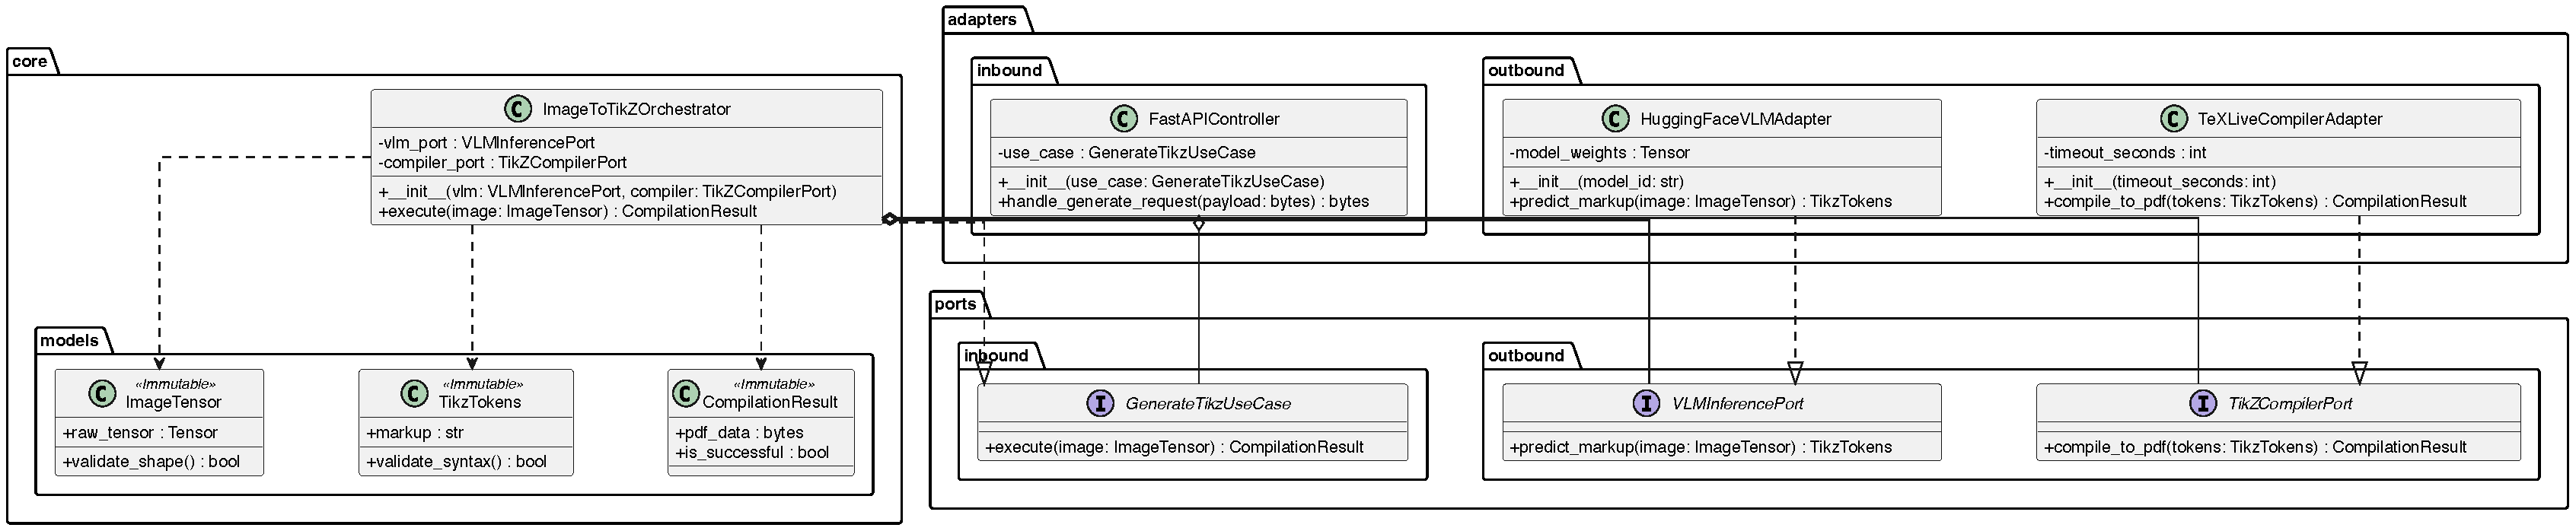
\includegraphics[width=0.95\linewidth]{../architecture/class_diagram.pdf}
    \caption{Class Diagram illustrating the Core Abstractions}
\end{figuresrswide}
\end{landscape}


\section{Multithreading}

The primary limitation of \(\mathcal{O}(1)\) sequential simulation is raw CPU clock speed. However, because each simulated price trajectory is completely independent of the others in the Monte Carlo framework, the architecture can scale across all available CPU cores.We also avoid using synchronization mechanisms like semaphores or mutex. Instead, the design relies on:
\begin{enumerate}
    \item \textbf{Local Isolation \& RNG Reliability:} Each thread instantiates its own isolated Pseudo-Random Number Generator (\texttt{std::mt19937\_64}) \cite{matsumoto1998mersenne}. To guarantee statistically independent sample paths, the main thread orchestrates a deterministic cryptographic-style avalanche hash function (combining the root seed with the thread ID) to uniquely seed each worker. This master-worker seeding architecture explicitly avoids concurrent calls to \texttt{std::random\_device} across threads, eliminating the risk of OS entropy pool exhaustion or deterministic lockups found in certain compiler implementations.
    \item \textbf{L1/L2 Cache Coherence (False Sharing Mitigation):} During the \(\mathcal{O}(N)\) simulation loop, each thread accumulates its payoff sum in a local stack variable (\texttt{localSum}). It is only upon loop completion that the thread writes its aggregated result to a unique index in the global \texttt{std::vector} (\texttt{partialSums[threadId]}). By avoiding continuous writes to adjacent memory addresses during the hot loop, the architecture mathematically prevents race conditions. This design conforms to MESI cache coherence protocols \cite{hennessy2011computer}.
    \item \textbf{Implicit Synchronization:} The main execution thread spawns the workers and immediately calls \texttt{join()}, so the total payoff is aggregated only after all threads have fully resolved.
\end{enumerate}

\begin{figuresrs}[red!5!white]
    \includegraphics[width=0.87\textwidth]{../architecture/sequence_diagram.pdf}
    \caption{Sequence Diagram of the Multithreaded Execution Flow}
\end{figuresrs}
\clearpage
\section{Mathematical Accelerator: Antithetic Variates}

Beyond hardware parallelism, the engine incorporates \textbf{Antithetic Variates}, a variance reduction technique that fundamentally accelerates the convergence of the Monte Carlo estimator.

For each generated standard normal variable \(Z \sim \mathcal{N}(0,1)\), we analytically evaluate two symmetric paths simultaneously using both \(Z\) and its perfect negative correlate \(-Z\). If \(V(Z)\) is the payoff using the noise \(Z\) and \(V(-Z)\) using its antithesis, the antithetic estimator is defined as \(\hat{V}_{AV} = \frac{V(Z) + V(-Z)}{2}\).

The variance of this estimator can be formally expanded as:
\begin{equation}
\text{Var}(\hat{V}_{AV}) = \frac{1}{4} \left( \text{Var}(V(Z)) + \text{Var}(V(-Z)) + 2\text{Cov}(V(Z), V(-Z)) \right)
\end{equation}

Since the paths are drawn from the same underlying distribution, \(\text{Var}(V(Z)) = \text{Var}(V(-Z)) = \sigma^2\). The equation simplifies to:
\begin{equation}
\text{Var}(\hat{V}_{AV}) = \frac{\sigma^2}{2} + \frac{1}{2}\text{Cov}(V(Z), V(-Z))
\end{equation}

Because standard option payoff functions (e.g., \(\max(S_T - K, 0)\)) are monotonic with respect to the underlying noise \(Z\), the covariance \(\text{Cov}(V(Z), V(-Z))\) is inherently negative. This negative covariance is the stochastic engine that mathematically guarantees \(\text{Var}(\hat{V}_{AV}) < \frac{\sigma^2}{2}\). Therefore, this technique not only halves the number of expensive invocations required from the C++ random number generator (\texttt{std::mt19937\_64})---doubling effective hardware bandwidth---but it ensures a reduction in standard error compared to crude Monte Carlo \cite{glasserman2004monte}.

\section{Computational Bridge (pybind11)}

The C++ and Python boundary is bridged via \texttt{pybind11}. This integration acts as the computational bridge, exposing the C++ OOP classes (\texttt{EuropeanOption}, \texttt{MarketData}, and \texttt{MonteCarloPricer}) directly to Python as native objects.

Beyond mere memory translation, this boundary acts as a strict validation layer. Invalid parameters provided at the Python level (e.g., negative volatility or negative time-to-maturity) trigger native C++ exceptions (\texttt{std::invalid\_argument}). \texttt{pybind11} automatically captures and safely propagates these as standard Python \texttt{ValueError} exceptions. This guarantees that the C++ backend operates exclusively under mathematically valid assumptions, preventing silent runtime failures.

Because \texttt{pybind11} translates C++ pointers and memory structures to Python without enforcing deep copies (\textit{zero-copy} architecture), data transfer latency is minimized. Python acts purely as the high-level orchestrator for research and data visualization, delegating all $\mathcal{O}(N)$ computational loops to the compiled binary.
